\section{OpenNMS Community}
The \emph{OpenNMS} community is a global community consisting of developers, corporations, service providers, researchers and users.

\subsection*{Role of \emph{The OpenNMS Group}}
One of the biggest part of code and project contribution is made by \emph{The OpenNMS Group, Inc.} The \emph{OpenNMS Group} build a business and builds a bridge to get the software \emph{OpenNMS} as 100\% free software into commercial companies and help with development and support. The \emph{OpenNMS Group} becomes the main driver for the free software OpenNMS. They run and provide the infrastructure for:
\begin{itemize}
  \item Continous integration to build, test, compile and deploy OpenNMS.
  \item Packaging and providing infrastructure distributing pre-compiled packages for different operating systems and \emph{Linux/Unix} distributions
  \item Public issue tracking for bugs, enhancements and feature requests
  \item Providing and running public mailing lists
  \item Maintaining the software branches and source code repository
  \item Software release management
\end{itemize}

\subsection*{Order of the Green Polo}
The secret brotherhood of OpenNMS.

\subsection*{OpenNMS Foundation Europe}
To cover non-commercial interests the \emph{OpenNMS Foundation Europe e.V.} (OFE) was founded in July 31st. in Fulda, Germany. It is a registered non-profit organization in Germany. The objective of the organization is to promote the use and development of free open source software, especially \emph{OpenNMS} the research and education around free open source software and network (management) technologies. To do this, the \emph{OFE} organizes conferences and trainings and acts as an advocate for free open source software. The \emph{OFE} initiates software development and studies which are made available to the public under the \emph{GPL}\footnote{GNU General Public License: \url{http://www.gnu.org/licenses/gpl.html}} or a suitable successor.

\subsection*{Your Contribution to OpenNMS}
If you are a developer who would like to contribute to OpenNMS, you have to sign the \emph{OpenNMS Contributor Agreement}. You can find the agreement at the following link \url{http://www.opennms.org/wiki/Contributor_Agreement}. The source code is hosted on \emph{github}. Code contributions can be merged into \emph{OpenNMS} with \emph{pull requests}. The workflow to get your source code into \emph{OpenNMS} is shown in picture \ref{fig:contrib-workflow} on page \pageref{fig:contrib-workflow}.
\begin{figure}
	\centering
	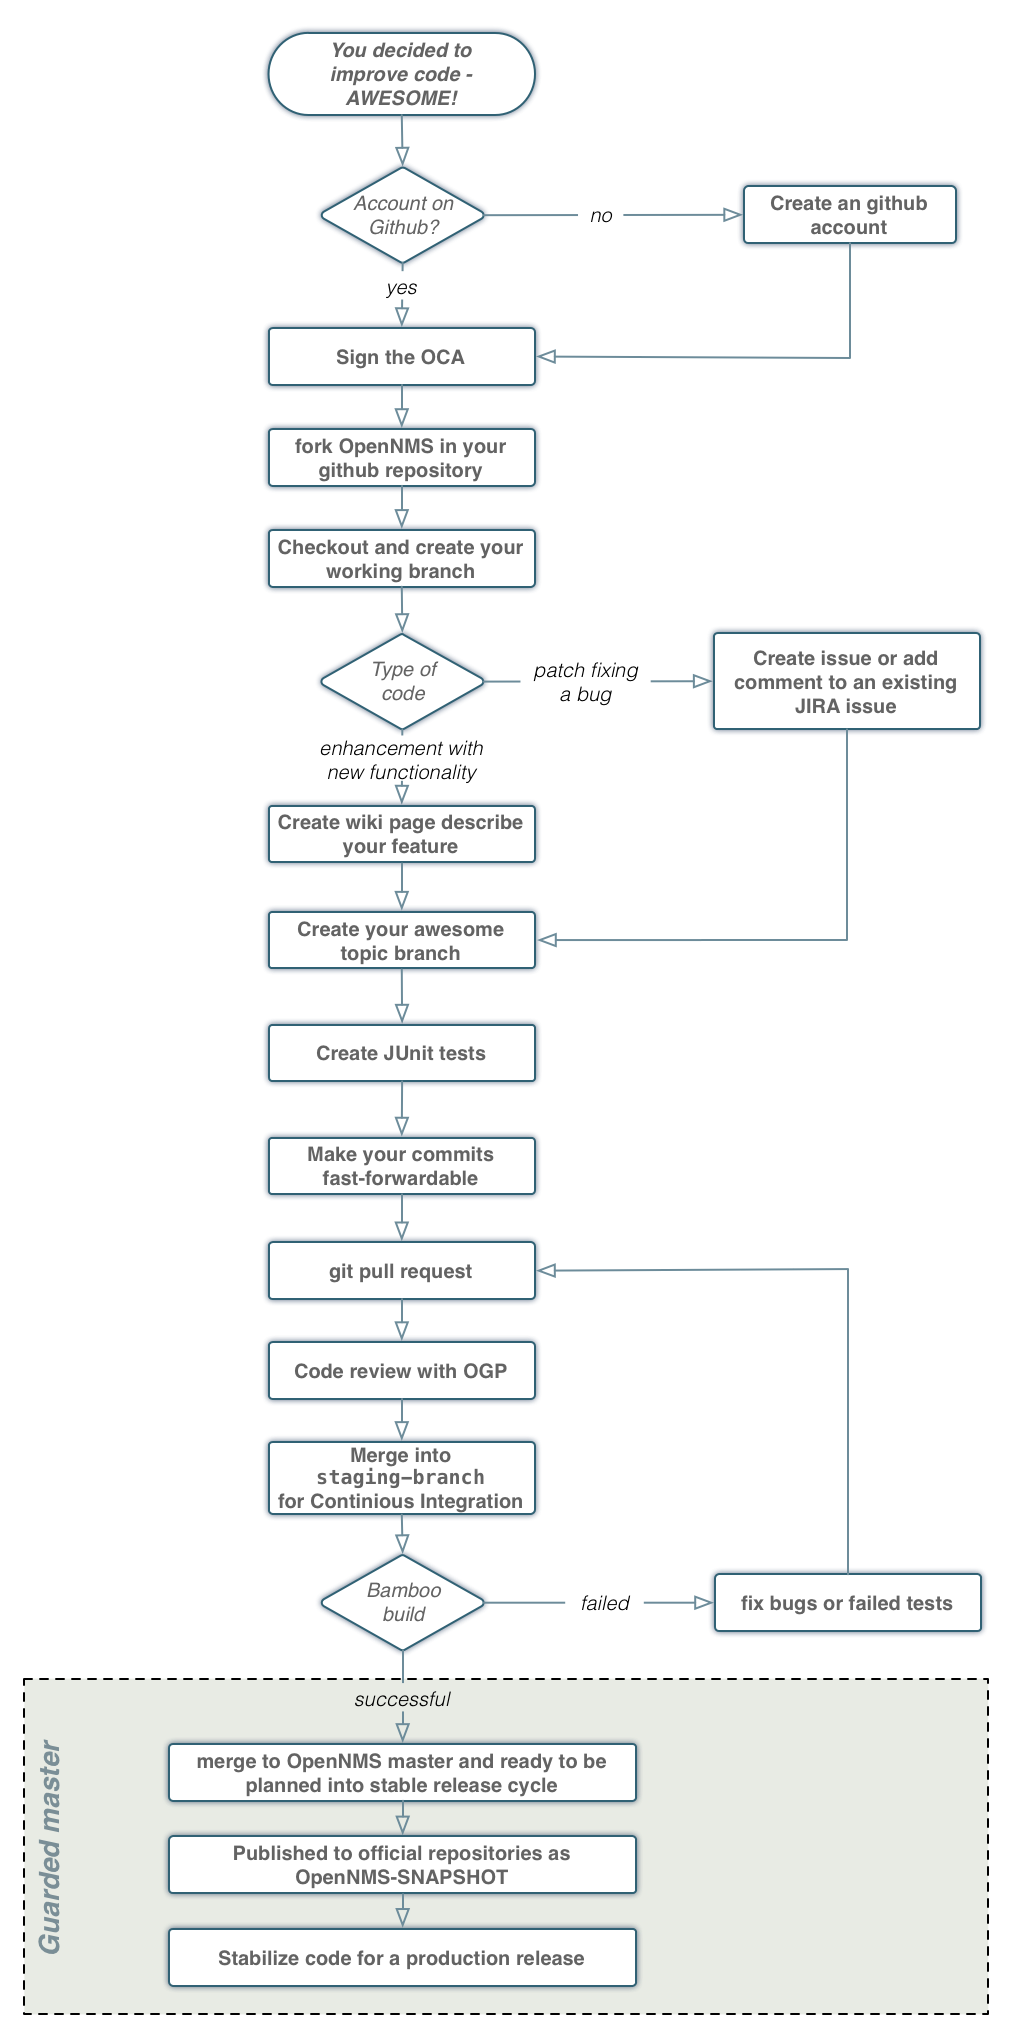
\includegraphics[width=0.75\textwidth]{images/contribution-workflow.png}
	\caption{Workflow for code contribution}
	\label{fig:contrib-workflow}
\end{figure}

\subsection*{Get your IDE up and running}
The \emph{OpenNMS} project is written in \emph{Java}. To maintain and handle external libraries it uses \emph{Maven}. It contains even more advanced technologies like \emph{OSGi} for class loading and \emph{Vaadin} as user interface framework. As version control system the project uses \emph{git}. To get an introduction working with \emph{git} and get your development environment up and running you can find documentation on the following wiki pages:
\begin{itemize}
  \item \url{http://www.opennms.org/wiki/Developing_with_Git}
  \item \url{http://www.opennms.org/wiki/Eclipse_and_OpenNMS}
\end{itemize}

\subsection*{Issue tracking, code browser and build system}
To document bugs, enhancements and feature request, the \emph{OpenNMS Group, Inc.} provide and maintains a public \emph{Atlassian JIRA} installation. It is recommended you create your JIRA account, which allows you to document bugs, enhancements or feature requests. The application for issue and feature tracking is available on \url{http://issues.opennms.org}.

The \emph{OpenNMS} software development follows a test driven approach. To provide a stable and continous quality of the code base, the \emph{OpenNMS Group} provides and run \emph{Atlassian Bamboo} as a build system. It compiles, tests and deploys the \emph{OpenNMS} software from the public \emph{git} repositories. The build system is public available on \url{http://bamboo.internal.opennms.com:8085}.

\emph{The OpenNMS Group} provides public access to \emph{Atlassian Fisheye} which gives the possibility to browse code from a browser and search for commit messages. The code browser is available on \url{http://fisheye.opennms.org}.